\documentclass{../source/Experiment}

\major{信息工程}
\name{}
\title{多层神经网络训练}
\stuid{}
\college{信息与电子工程学院}
\date{\today}
\lab{教11-400}
\course{人工智能实验}
\instructor{胡浩基、魏准}
\grades{}
\expname{多层神经网络训练}
\exptype{设计验证}
\partner{}
\begin{document}
\makecover
\section{实验题目}
\subsection{实验5-2}

通过SGD训练方法、Sigmoid激活函数及BP规则,对上述神经网络进行训练,并输出训练后的结果。

利用实验5-1(上节课)的单层网络及SGD方法,用上述数据进行训练并测试,查看并对比两种网络输出结果,分析原因;

\subsection{实验5-3}

将神经网络更新规则改为momentum,对上述神经网络进行训练,输出训练后的结果,比较不同$\beta$值momentum训练方法及不用momentum训练方法时,误差(真实结果与输出的MSE)随epoch变化趋势,并可视化结果

\section{实验结果}
\subsection{实验5-2}
可视化结果
\begin{figure}[H]
    \centering
    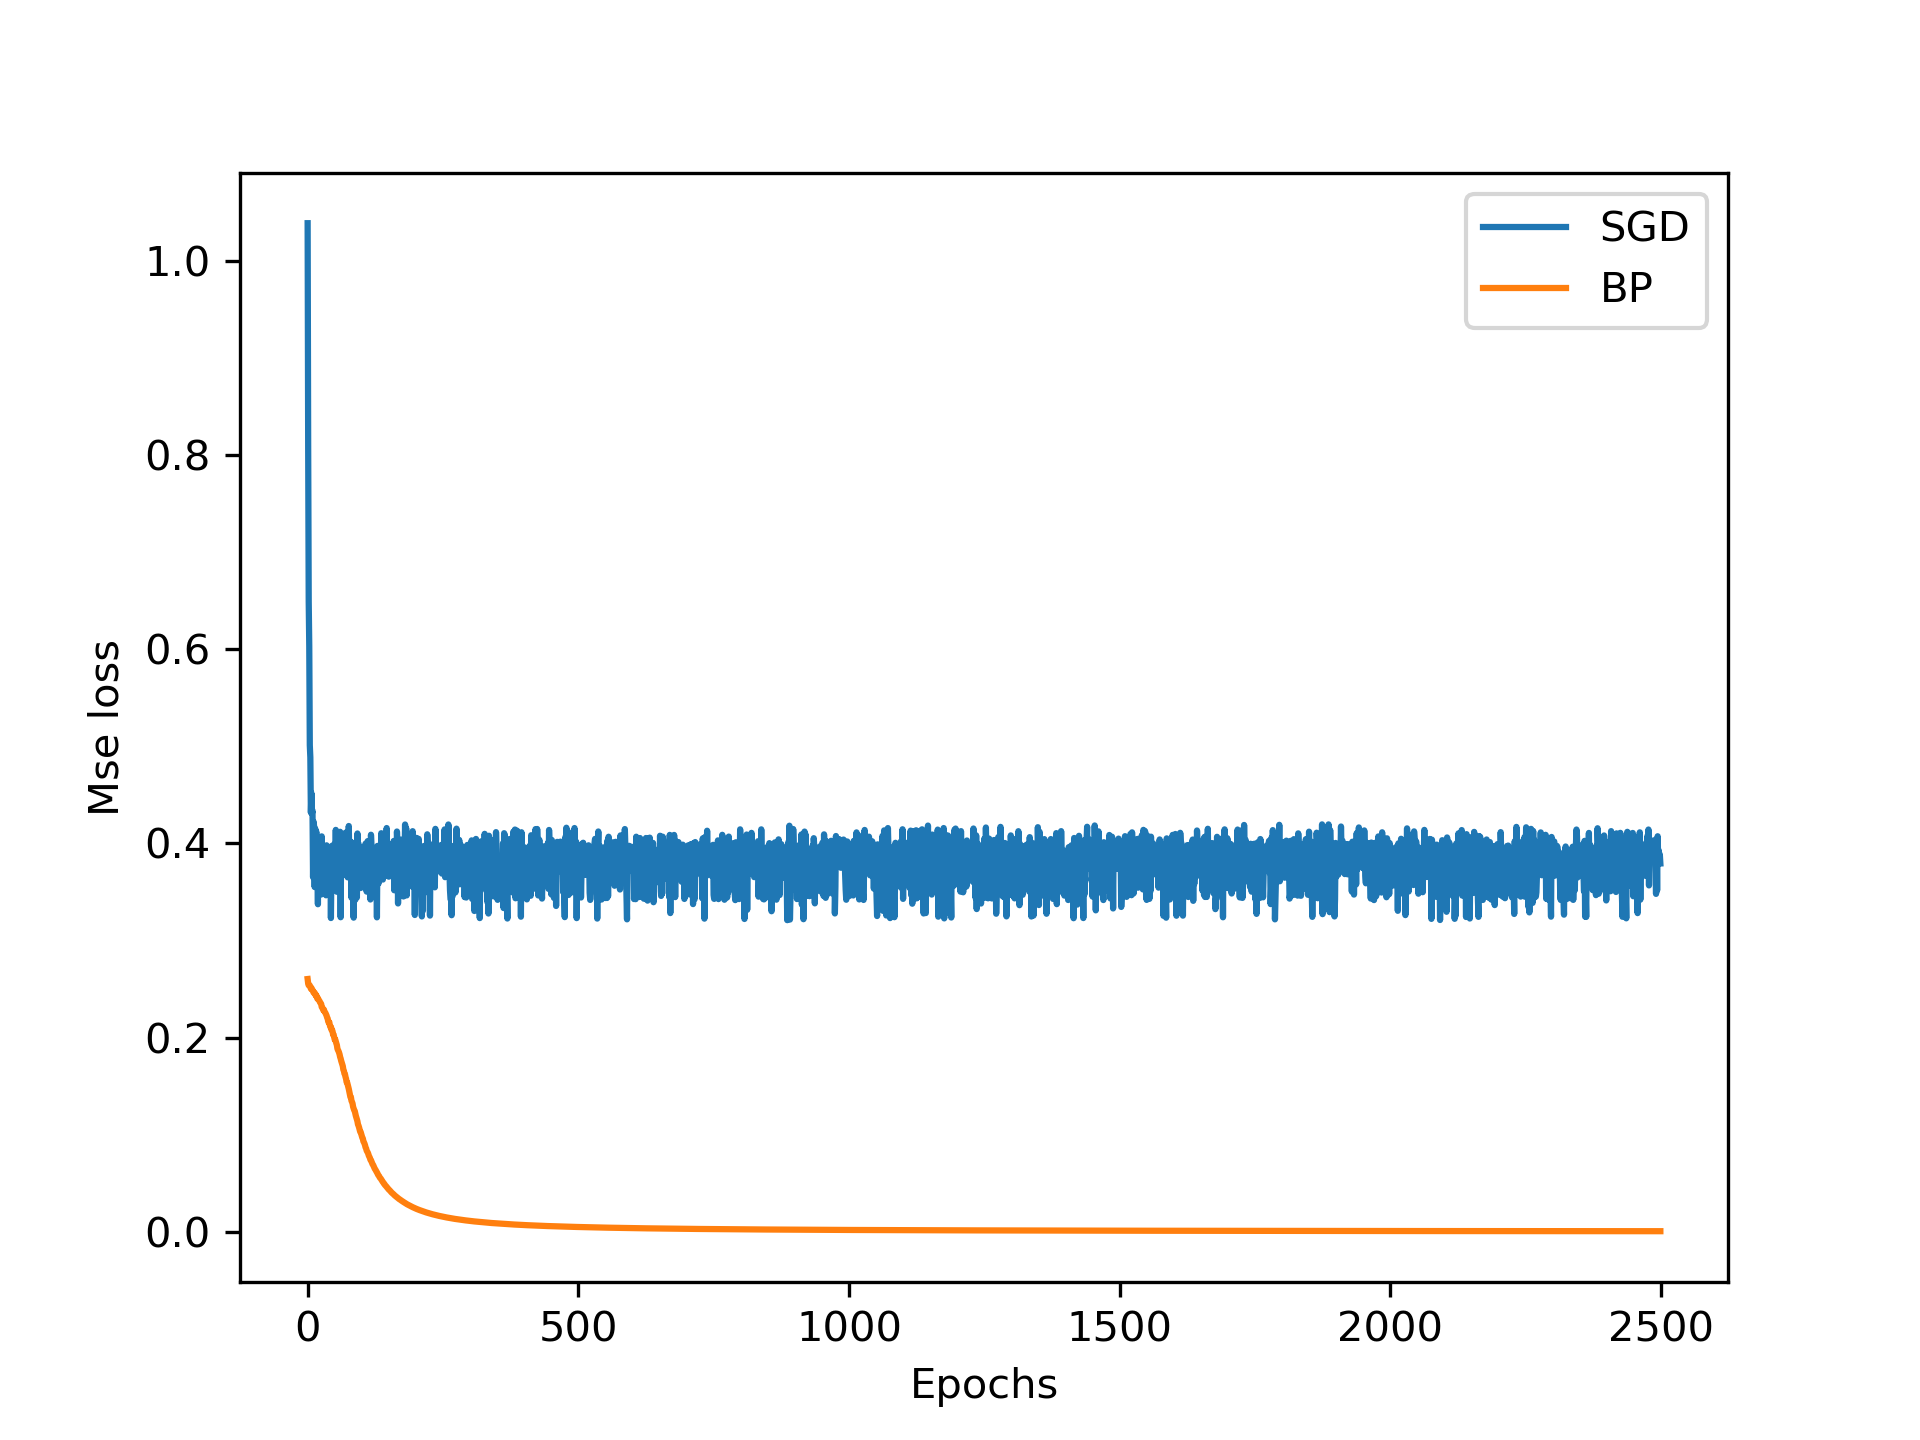
\includegraphics[width = 0.6\textwidth]{Part5/参考/lab5_2.png}
    \caption{可视化}
\end{figure}

原因:单层网络无法实现异或

\subsection{实验5-3}
可视化结果
\begin{figure}[H]
    \centering
    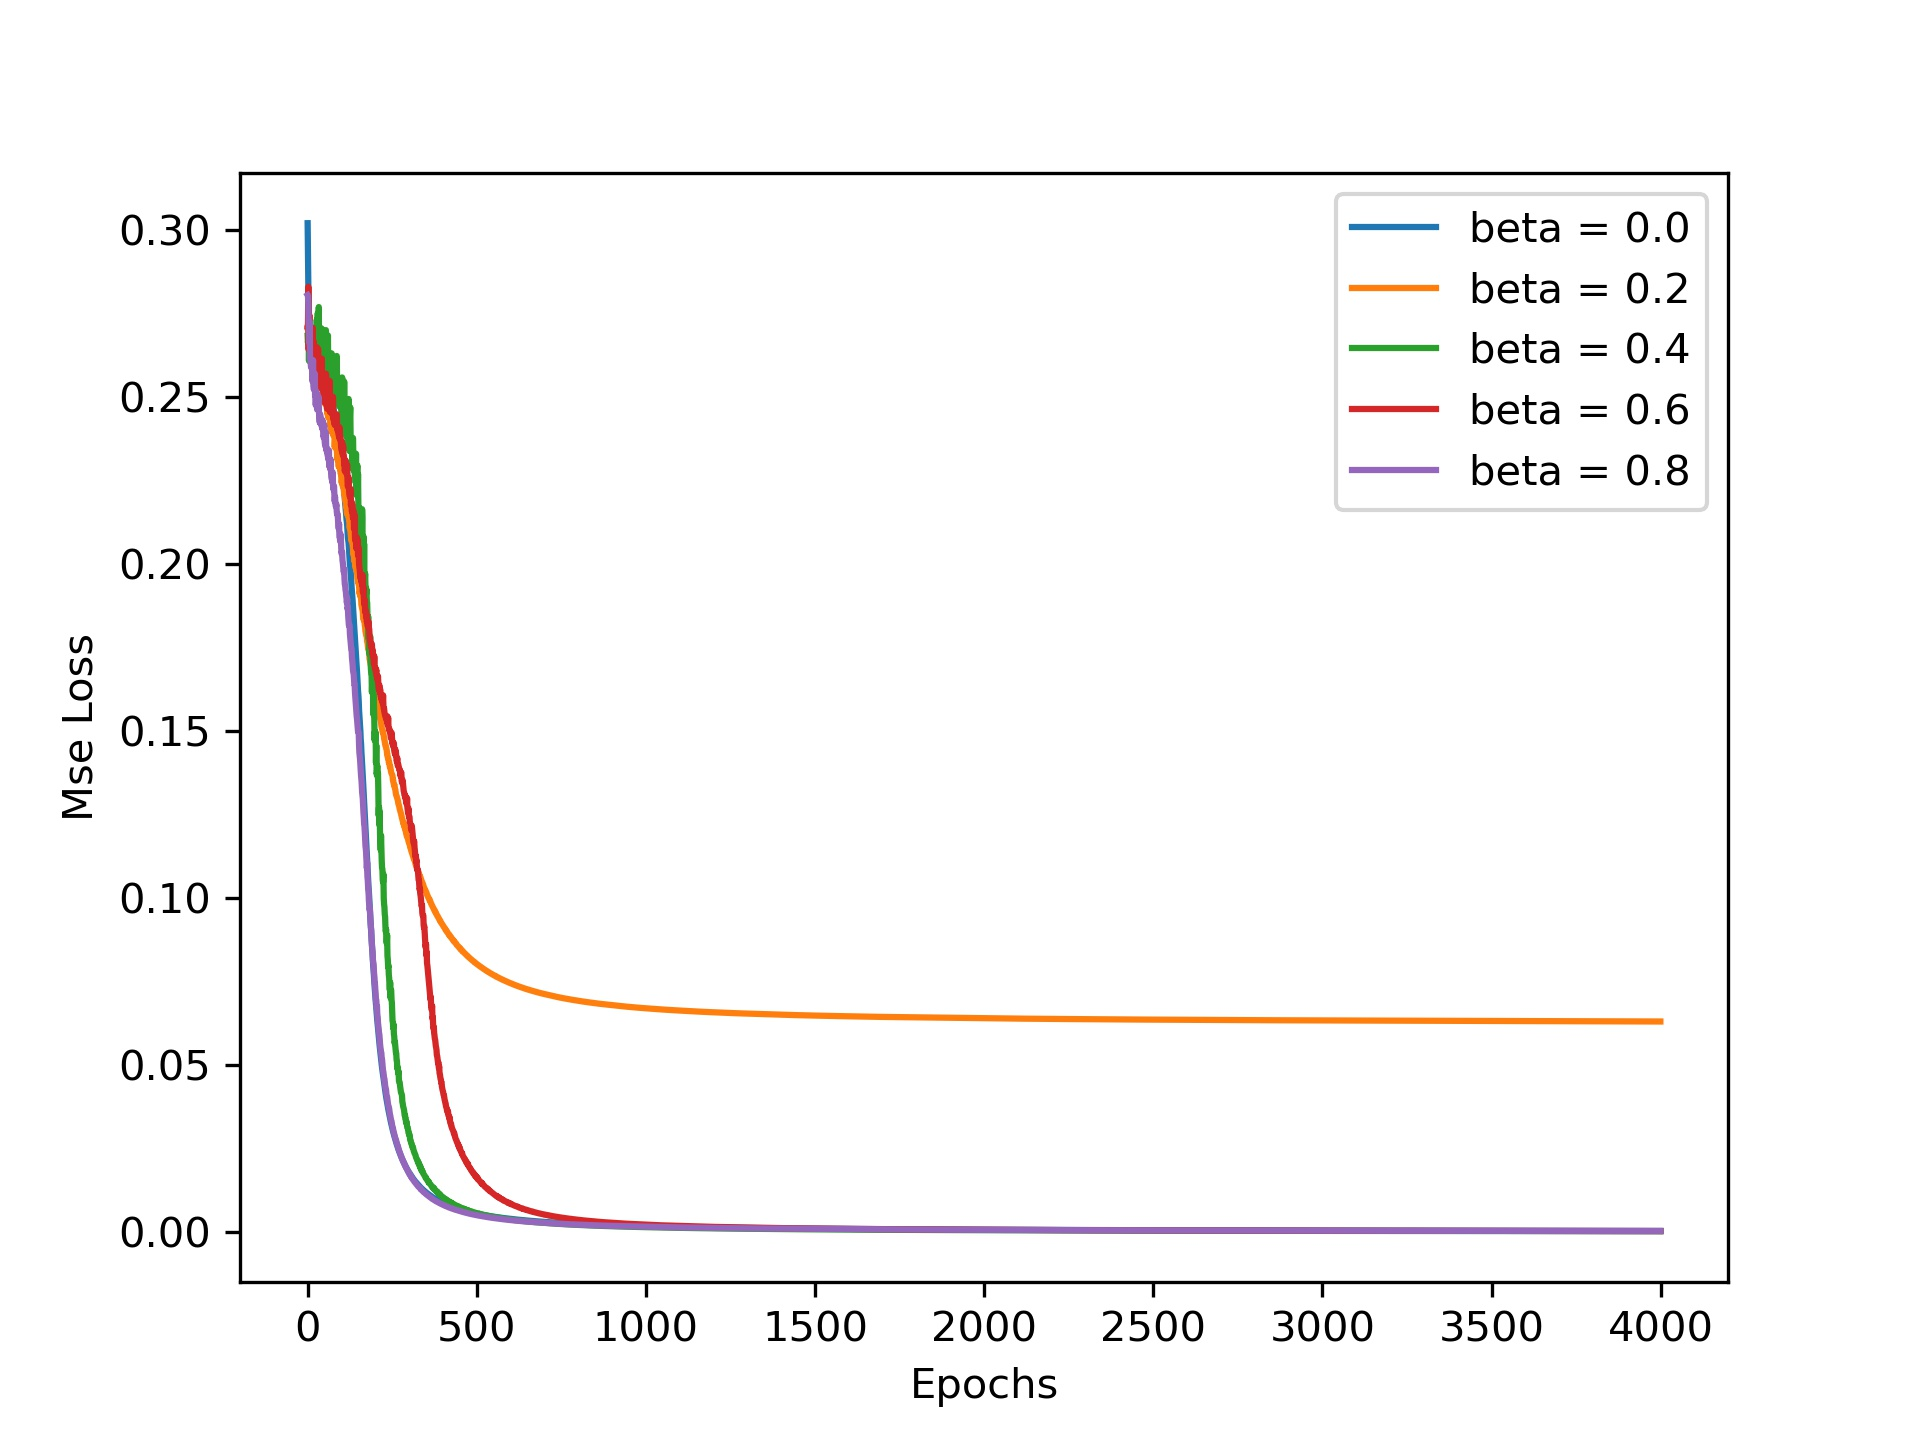
\includegraphics[width = 0.6\textwidth]{Part5/参考/lab5_3.jpg}
    \caption{可视化}
\end{figure}
\end{document}


